\chapter{Results}

In this chapter, the correctness and efficiency of the full algorithm and the effect of the optimizations were shown. The benchmark platforms are 3 personal computers with slightly heterogeneous hardware and operating systems. The following list showed the hardware and operating systems of the benchmark platforms.
\begin{enumerate}
  \item \textbf{PC1}: AMD Ryzen 7 4800U, 16GB RAM, Windows 10; running 2 workers
  \item \textbf{PC2}: AMD Ryzen 7 1700, 16GB RAM, Windows 10; running 2 workers
  \item \textbf{PC3}: AMD Ryzen 7 2700X, 32GB RAM, Windows 10; running 1 workers
\end{enumerate}
During testing, the cluster can generate a public key and corresponding distributed private keys correctly and efficiently. The generated public key can be printed in correct format and the information can be parsed correctly using 3rd party key parser. A message can be encrypted by the manager using the implemented encryption algorithm, and the encrypted message can be correctly decrypted by the workers using the distributed private keys.

\begin{figure}[htbp]
  \centering
  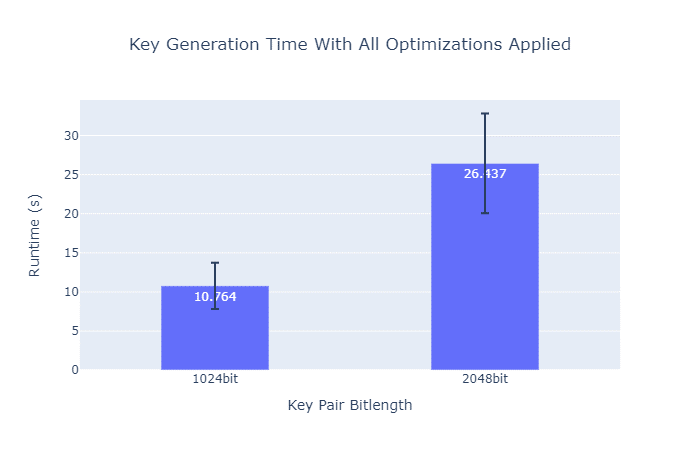
\includegraphics[width=.8\textwidth]{images/key_gen_time.png}
  \label{fig:key_gen_time}
  \caption{This figure shows the time required for key pair generation for keys with different bit length. On the tested platforms, the total generation time for a 1024-bit key is only 10 seconds, whereas the total generation time for a 2048-bit key is about 26 seconds.}
\end{figure}

\begin{figure}[htbp]
  \centering
  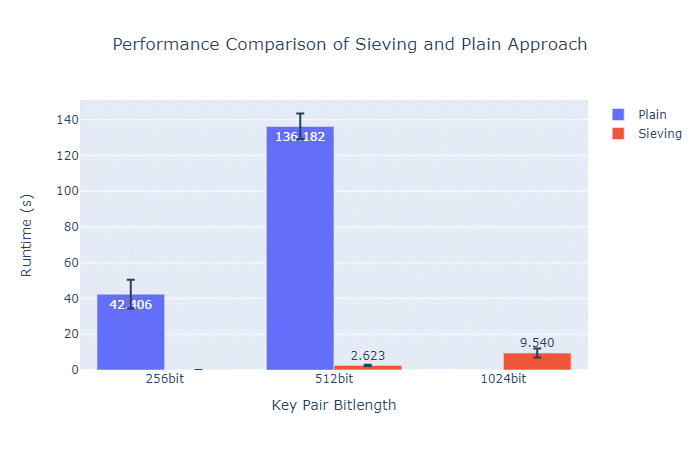
\includegraphics[width=0.8\textwidth]{images/comparison_sieving.png}
  \label{fig:sieving}
  \caption{This figure shows the effect of applying distributed sieving. Without applying distributed sieving, generation a merely 256-bit long RSA key pair took already 42 seconds, which is already slower than genearting a 4 times longer key pair with distributed sieving enabled. Generating a 512-bit key pair took more than 1.5 minutes, whereas the optimized version took no more than 3 seconds.}
\end{figure}

\begin{figure}[htbp]
  \centering
  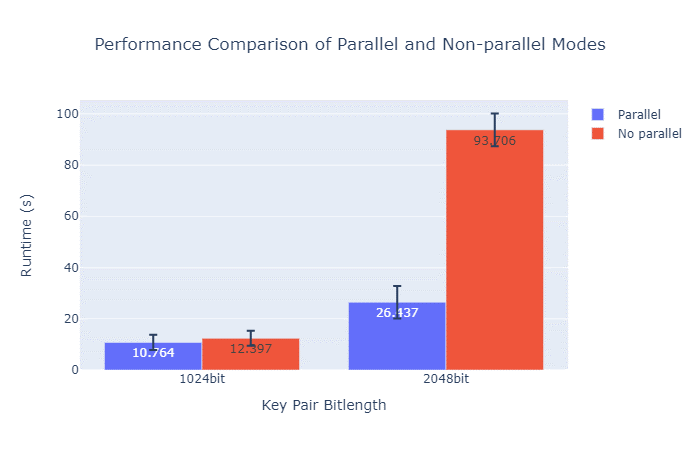
\includegraphics[width=0.8\textwidth]{images/comparison_parallel.png}
  \label{fig:parallel}
  \caption{This figure shows the effect of parallelization. The effect is conspicuous for 2048-bit long RSA keys. Without enabling parallelization, the generation of a 2048-bit long RSA key pair took about 1.5 minutes, whereas the optimized version took only half a minute.}
\end{figure}
